\chapter{General Addenda}

If there are several additions you want to add, but they do not fit into the thesis itself, they belong here.
\section{Other Related Work}
In the following sections several works in the domain adaption and PHM context are presented, which are mentioned several times thoughout the thesis. Since they are not closely related to the topic of the thesis they are described in the appendix

\subsection{Prognostics and Healthmanagement system for Rolling Bearings using a Maximum Mean Discrepancy Loss and Domain Classifier}
PHM of rolling bearing is a task with high demand in the industry. Guo et al \cite{Guo2019} propose a deep convolutional transfer learning network (DCTLN), which reduces the domain discrepancy by applying a MMD-loss and domain classifier. The architecture of the model is visualized in fig. \ref{fig:DCTLN_model}. Features are extracted by a CNN containing 16 layers including one input layer, six convolutional layers, six pooling layers, two fully connected layers, and one output layer. Each convolutional layer is combined with a consecutive pooling layer. The model three main training goals during optimization. A CE-loss ($L_{c}$) is applied to improve the prediction accuracy on the source domain data. The MMD metric ($\hat{D}$) is used to measure and reduce the domain discrepancy in the latent feature space and a domain classifier is trained to predict the corresponding domain for each sample. The  domain classification loss is defined as:
\begin{equation}
    L_{d} = \frac{1}{m} \sum_{i=1}^{m} (g_{i} log(d(x_{i})) + (1-g_{i}) log(1-d(x_{i})))
\end{equation}
The classifier is optimized solely with the source CE-loss and the domain classifier with the domain classification loss. The feature extractor is optimized with the three training goals in total:
\begin{equation}
    L = L_{c} + L_{d} + \hat{D}
\end{equation}

\begin{itemize}
    \item [\textbf{Objective 1}:] By minimizing the CE-loss the model training minimizes the health condition classification error on the source domain data.
    \item [\textbf{Objective 2}:] The domain classifier processes the features in the layer FC3 and tries to predict the corresponding domain of each sample. The model is trained to extract domain invariant features such that the error of the domain classifier is increased.
    \item [\textbf{Objective 3}:] By extracting more domain-invariant features the MMD-loss is reduced in the feature map FC2 \cite{Guo2019}. 
\end{itemize}


\begin{figure}[H]
  \centering
  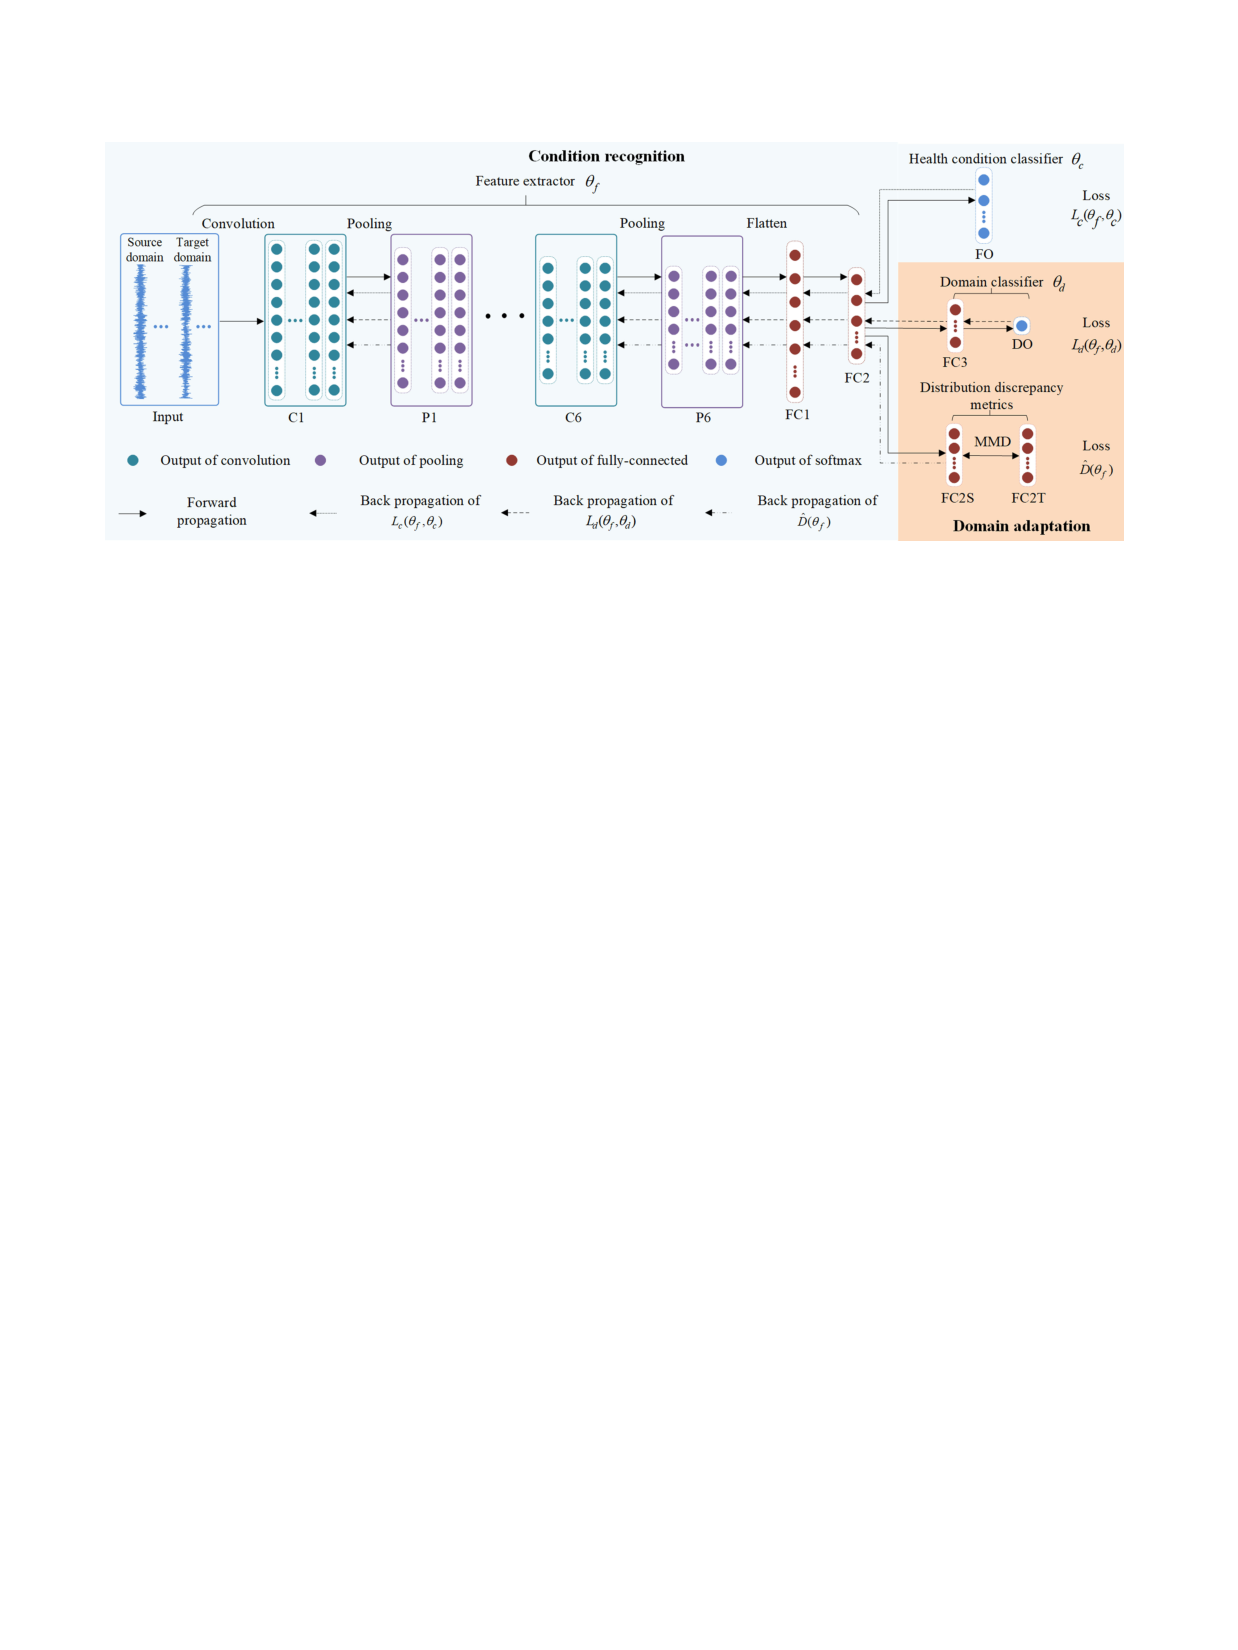
\includegraphics[width=1\textwidth]{models_state_of_the_art/DCTLN_model.pdf}
  \caption{DCTLN model proposed by Guo et al \cite{Guo2019}}
  \label{fig:DCTLN_model}
\end{figure}


\subsection{Wasserstein Distance Guided Multi-Adversarial Network for Prognostics and Healthmanagment for Rolling Bearings}
Zhang et al \cite{Zhang2019} present a Wasserstein distance guided multi-adversarial network (WDMAN) for rolling bearing fault diagnosis under different working conditions. The proposed architecture consists of a CNN feature mapper and a subsequent classifier. In the fully connected layers of the classifier, several Domain Critic Networks estimate the domain discrepancy by applying the Wasserstein-distance. A source CE-loss is applied in the end of the network. The whole model and the applied losses are visualized in fig. \ref{fig:WDMAN_model}.

 \begin{figure}[H]
  \centering
  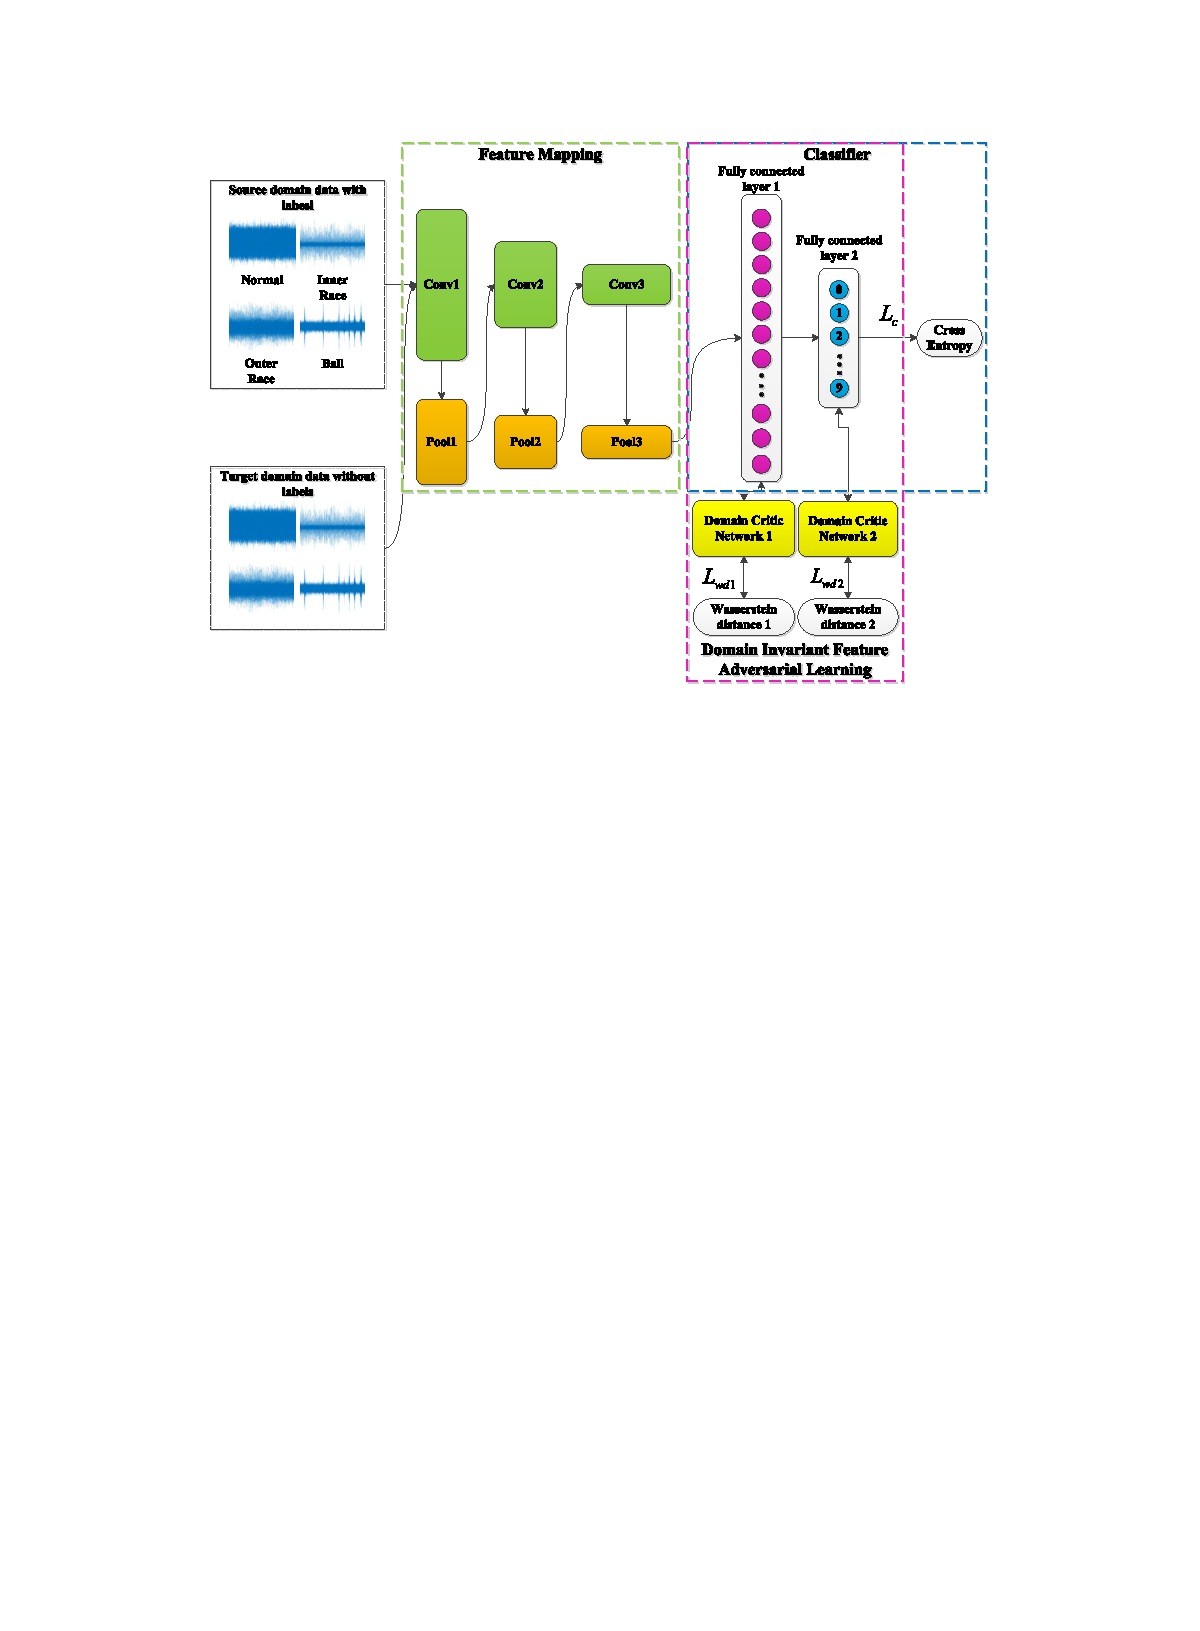
\includegraphics[width=1\textwidth]{models_state_of_the_art/WDMAN_model.pdf}
  \caption{WDMAN architecture proposed by Zhang et al \cite{Zhang2019}}
  \label{fig:WDMAN_model}
\end{figure}

In a pre-training phase, the feature mapper $\theta_{M}$ and classifier $\theta_{C}$ are optimized with the source CE-loss:
 
\begin{equation}
     L_{c}(x^{s}, x^{t}) = -\frac{1}{n^{s}} \sum_{i=1}^{n^{s}} \sum_{k=1}^{K} l(y_{i}^{s}=k) \cdot logC(M(x_{i}^{s}))_{k},
\end{equation}

where $n^{s}$ is the number of source samples, $K$ is the number of classes, $x_{i}^{s}$ and $y_{i}^{s}$ are the source samples and corresponding labels, $M(\cdot)$ and $C(\cdot)$ are the feature mapper and classifier. In the adversarial training afterwards, the model learns to extract more domain invariant features by minimizing the Wasserstein distance in the fully connected layers of the classifier. The domain critic networks try to maximize and the feature mapper to minimize the adversarial loss. The adversarial training transfers the model, trained on the source domain, to the target domain:
 
\begin{equation}
     L_{wd}(x^{s}, x^{t}) = \frac{1}{n^{s}} \sum_{x^{s} \in X^{s}} D(F(x^{s})) - \frac{1}{n^{t}} \sum_{x^{t} \in X^{t}} D(F(x^{t})),
\end{equation}

where $x^{s}$ and $x^{t}$ are the data samples drawn from the source domain $X^{s}$ and target domain $X^{t}$. The feature representations of the source and target samples in the fully connected layers are denoted as $F(\cdot)$. The domain critic networks are represented by $D(\cdot)$. In the adversarial learning, the model and discriminators are optimized in an alternating procedure:

\begin{equation}
    \min_{\theta_{F}} \max_{\theta_{D}} (L_{wd} - \lambda L_{gp}), 
\end{equation}

where $\theta_{F}$ and $\theta_{D}$ are the parameters of the feature mapper and domain critics, $\lambda$ is the penalty coefficient. Generally, the goal of the discriminators is to identify the domain of each sample. The feature mapper tries to extract domain-independent features, which precludes the discriminator predicting the correct domain. To satisfy the Lipschitz constraint condition of the Wasserstein distance, an additional gradient penalty is applied: 

\begin{equation}
     L_{gp}(\tilde{x}) = (|\nabla_{\tilde{x} \in P_{\tilde{x}}} D(\tilde{x})|_{2}-1)^{2}, 
\end{equation}
where $P_{\tilde{x}}$ is a distribution of samples coming from the line connecting a pair of points sampled from the source and target domain. The Wasserstein distance is extended with the gradient penalty. The workflow of the model is described more detailed in fig. \ref{fig:WDMAN_workflow}
 
\begin{figure}[H]
  \centering
  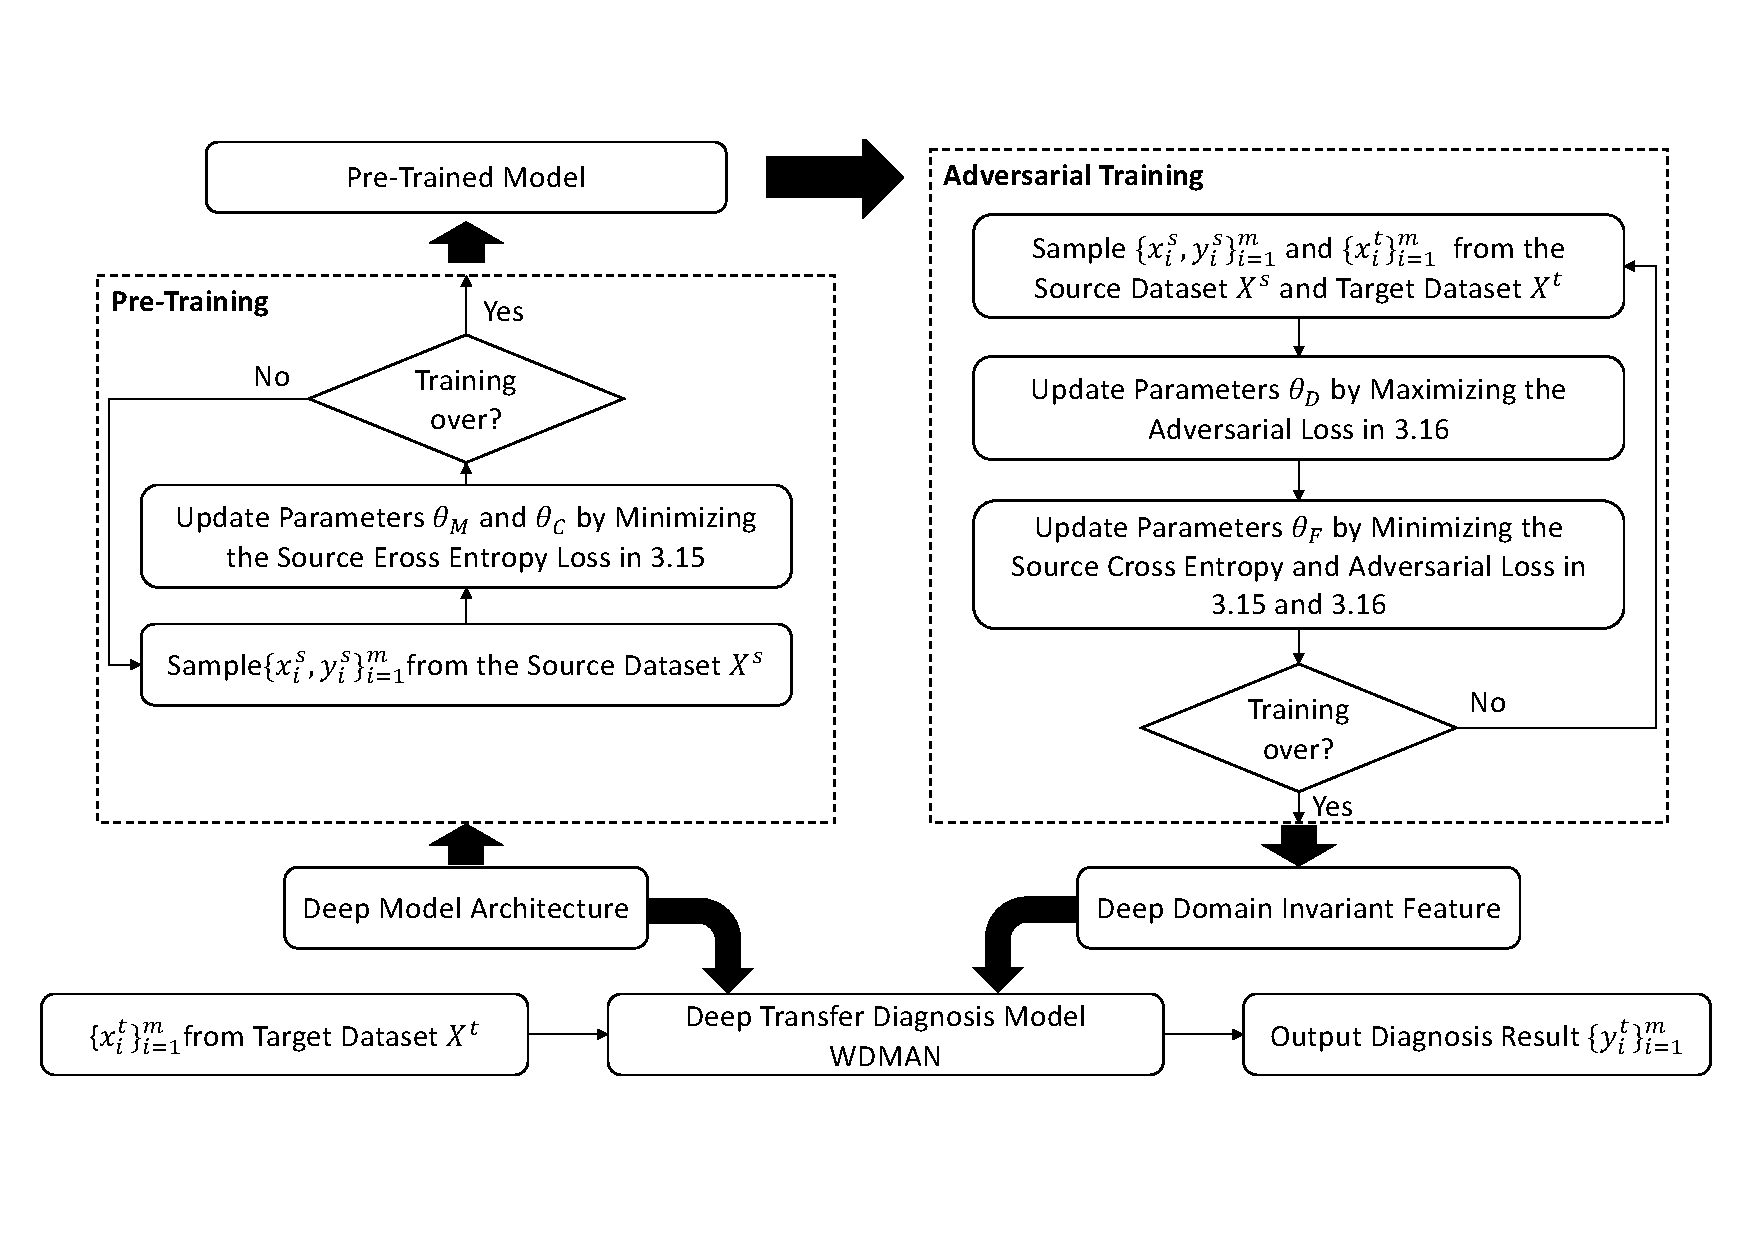
\includegraphics[width=.9\textwidth]{models_state_of_the_art/WDMAN_workflow.pdf}
  \caption{WDMAN workflow based on \cite{Zhang2019}}
  \label{fig:WDMAN_workflow}
\end{figure}
 
 

Even sections are possible, but usually only used for several elements in, e.g.\ tables, images, etc.

\chapter{Figures}
\section{Example 1}
\cmark
\section{Example 2}
\xmark